\documentclass[11pt]{article}
\usepackage[top=0.75in, bottom=0.75in, left=1in, right=1in]{geometry}
\usepackage{amsmath,amssymb,bbm}
\usepackage{amsthm}
\newtheorem{definition}{Definition}
\usepackage{graphicx}
\usepackage{subcaption}
\usepackage{microtype}
\usepackage[hidelinks]{hyperref}
\usepackage{grffile}

\title{\textbf{Neural-to-Rule Ensemble Distillation (NtRED)}\\[4pt]
\large A Cross-Paradigm Knowledge Distillation Framework}
\author{}
\date{}

\begin{document}
\maketitle
\vspace{-1.4em}

%% ─────────────────────────────────────────────────────────────
\section*{Framework Overview}

Classical knowledge distillation (KD) transfers compressed knowledge between neural networks: a
large teacher guides a smaller student through soft probability outputs---Hinton et al.'s ``dark
knowledge''~\cite{hinton2015}. Both parties remain within the neural paradigm; the student inherits
representational opacity from the teacher.

\textbf{NtRED} crosses the \emph{representational boundary}. The teacher is an ensemble of
large language models (LLMs); the student is a \emph{symbolic rule system}---any deterministic,
interpretable formalism such as grammar rules, logic predicates, or pattern-matching
expressions---illustrated in Figure~\ref{fig:kd_vs_ntred}. Both parties extract \emph{structures}
from documents: typed, identifiable units of content (e.g., a definition, theorem, or equation).
The objective is to transfer sufficient knowledge from the teacher ensemble into the student such
that, once distillation is complete, the student operates fully independently: no LLM is invoked
at inference time. This yields a computationally efficient, auditable system whose rules can be
inspected and extended by domain experts.

\begin{figure}[h]
  \centering
  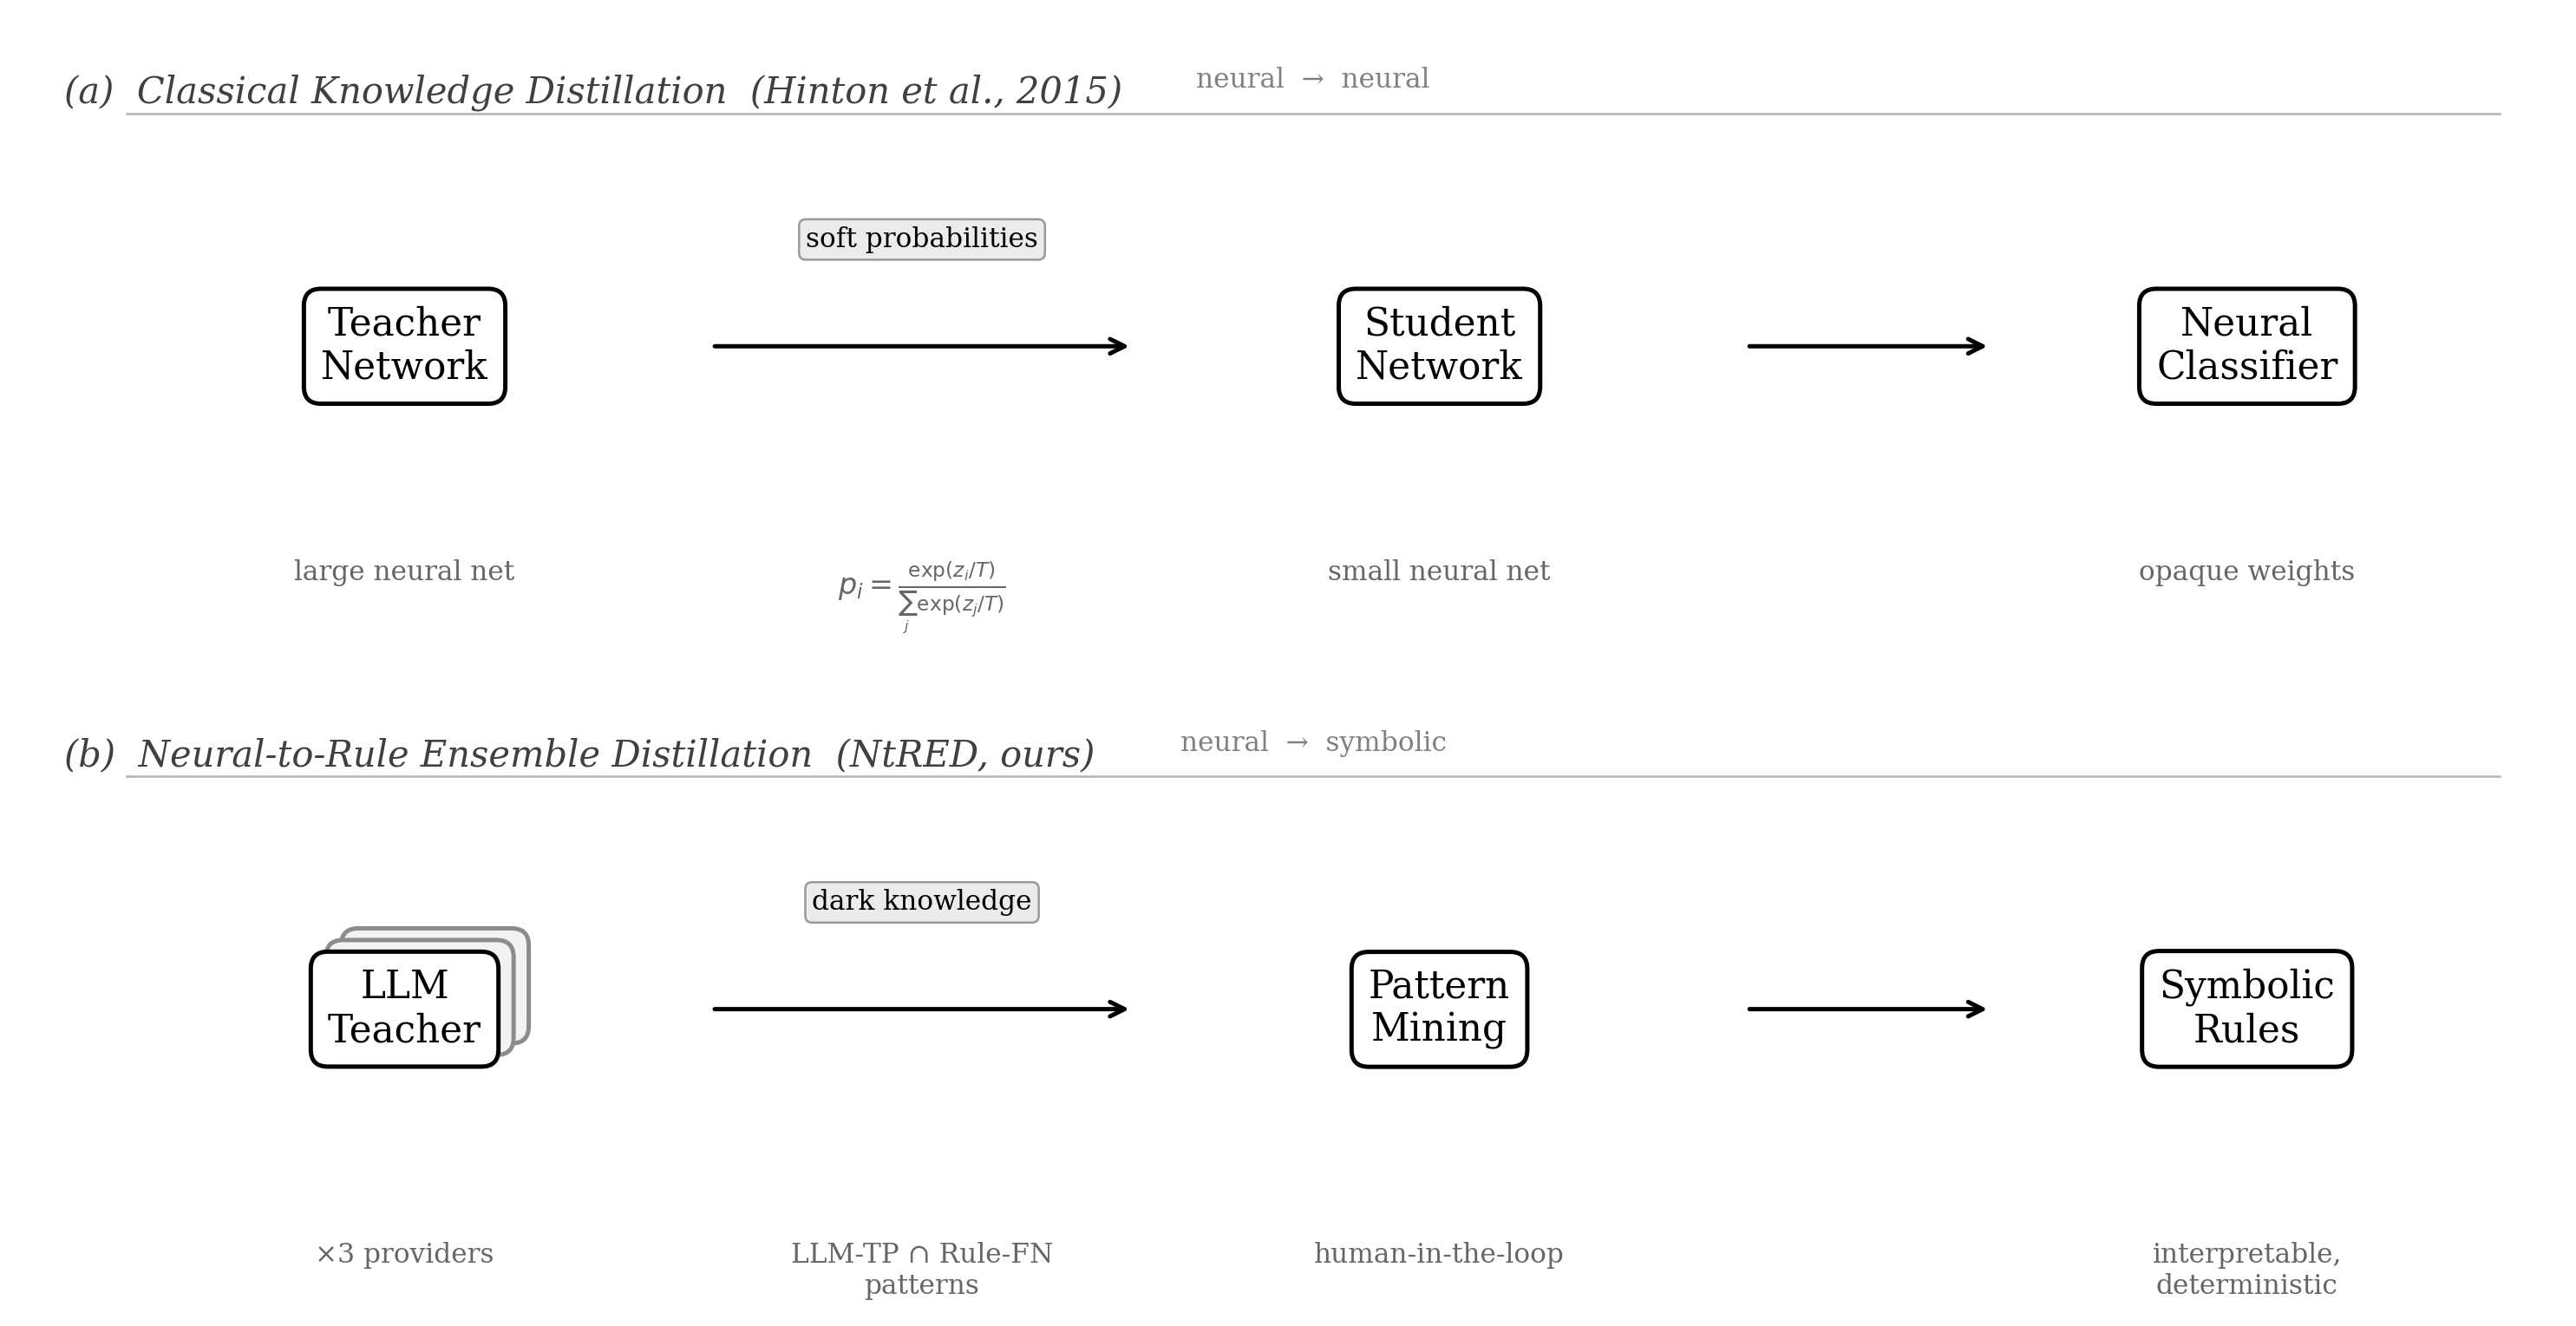
\includegraphics[width=0.88\textwidth]{kd_vs_ntred.png}
  \caption{Classical KD vs.\ NtRED. Classical KD transfers soft probabilities between two neural
    networks. NtRED crosses the representational boundary: the student is a fully interpretable
    symbolic rule system.}
  \label{fig:kd_vs_ntred}
\end{figure}

The framework proceeds in two phases. In \textbf{Phase~I}, each LLM teacher's extraction prompt
is optimised against a small gold-standard corpus (a manually annotated set of documents with
known-correct extractions) so that teacher outputs serve as reliable signals before distillation
begins. In \textbf{Phase~II}, the optimised teachers are run on a target corpus---labelled or
unlabelled---and the structures they detect that the symbolic student misses constitute the
\emph{dark knowledge} of the ensemble (we adopt this term from Hinton et al.\ to denote the
analogous gap in NtRED: the portion of the teachers' understanding not yet expressible by the
student's rules). These instances are mined to produce concrete updates to the student's rule set.

%% ─────────────────────────────────────────────────────────────
\section*{Phase I\,: Teacher Optimisation}

Before distillation, each LLM teacher's extraction prompt is iteratively refined against the
gold-standard corpus. Each iteration proceeds as follows: (i)~all providers independently extract
structures from the training documents, (ii)~extractions are evaluated against gold via
Jaccard-based F1, (iii)~a meta-LLM---a separate model that rewrites the extraction prompt
based on error analysis---analyses the false positives, false negatives, and
near-misses (partial matches below threshold~$\theta$) to produce a revised prompt.
Optimisation terminates when validation F1 on a held-out set plateaus
(Figure~\ref{fig:pipeline}). This step raises teacher quality prior to distillation,
ensuring that the signals propagated to the student are as accurate as possible.

\paragraph{Similarity measure.}
Matches between an extracted structure $s$ and a gold-standard entry $g$ are determined by
token-set Jaccard similarity. Let $T(\cdot)$ denote the set of tokens obtained after
normalising the text (lowercasing, collapsing whitespace) and tokenising into words, numbers,
and domain-specific symbols. The Jaccard similarity is:
%
\begin{equation}
  J(s,\, g)
    = \frac{\bigl|T(s) \cap T(g)\bigr|}{\bigl|T(s) \cup T(g)\bigr|}.
  \label{eq:jaccard}
\end{equation}
%
\begin{definition}[Match]
  A prediction $s$ is a \emph{match} for gold entry $g$ if $J(s, g) \geq \theta$, with
  default threshold $\theta = 0.7$.
\end{definition}
Precision, recall, and F1 are then computed over the resulting matched/unmatched sets in
the standard way.

%% ─────────────────────────────────────────────────────────────
\section*{Phase II\,: Distillation---Dark Knowledge and Rule Mining}

\paragraph{Dark knowledge.}
For a structure $s$ and an extractor $e$ (either a provider $p$ or the rule set
$\mathcal{R}^{(t)}$), let $\hat{y}_{e}(s) = 1$ if $e$ produces a match for $s$---i.e., some
output $s'$ with $J(s,s') \geq \theta$---and $0$ otherwise.
A structure is a \emph{false negative} (FN) for the student when its rules fail to match it,
and a \emph{true positive} (TP) for a teacher when the teacher successfully identifies it.

\begin{definition}[Dark Knowledge]
  A structure $s \in \mathcal{G}$ is \emph{dark knowledge} in NtRED at iteration $t$ if the
  student fails to match it ($\hat{y}_{\mathcal{R}^{(t)}}(s) = 0$) and at least one teacher
  recovers it ($\exists\, p \in \mathcal{P} : \hat{y}_{p}(s) = 1$). The dark knowledge set
  is the gap between what the current symbolic rules can express and what the LLM ensemble
  understands.
\end{definition}

Formally, let $\mathcal{G}$ be the gold-standard set of known structures, $\mathcal{P}$ the
teacher ensemble, and $\mathcal{R}^{(t)}$ the symbolic student rule set at iteration $t$:
%
\begin{equation}
  \mathcal{D}_{\mathrm{dark}}^{(t)}
    = \bigl\{\, s \in \mathcal{G}
        \;\big|\;
        \underbrace{\hat{y}_{\mathcal{R}^{(t)}}(s) = 0}_{\text{student FN}}
        \;\wedge\;
        \underbrace{\exists\, p \in \mathcal{P} : \hat{y}_{p}(s) = 1}_{\text{teacher TP}}
      \bigr\}.
\end{equation}
%
\paragraph{Extension to unlabelled corpora (Discovery Mode).}
When no gold standard is available---as is typical for large-scale corpora---distillation
can still proceed by replacing the gold signal with teacher consensus. If at least $\tau = 2$
independent teachers agree on a candidate structure, it is treated as a reliable positive
(a stricter requirement than distillation mode, since no human annotation backs it):
%
\begin{equation}
  \mathrm{consensus}(s)
    = \mathbbm{1}\!\left[\;\sum_{p \in \mathcal{P}} \hat{y}_{p}(s) \;\geq\; \tau\;\right],
    \qquad \tau = 2.
\end{equation}
%
The two operating modes are contrasted in Figure~\ref{fig:venn}. Mined candidates are
reviewed and incorporated into the student rule set, allowing distillation to scale to any
unlabelled corpus.

\paragraph{Rule update loop.}
For each instance in $\mathcal{D}_{\mathrm{dark}}^{(t)}$, a dedicated LLM
inspector---distinct from both the extraction teachers and the Phase~I meta-LLM---receives the
current student implementation together with the surrounding document context and proposes a
concrete rule update. Proposed rules are reviewed and incorporated into the student:
%
\begin{equation}
  \mathcal{R}^{(t+1)}
    = \mathcal{R}^{(t)} \;\cup\; \Delta\mathcal{R}^{(t)},
  \qquad
  \Delta\mathcal{R}^{(t)} = \mathrm{PatternMine}\!\left(\mathcal{D}_{\mathrm{dark}}^{(t)}\right),
\end{equation}
%
where $\mathrm{PatternMine}$ denotes the LLM-inspector-driven rule-synthesis step above.
The loop terminates when $\mathrm{F_1}(\mathcal{R}^{(t+1)}) \approx \mathrm{F_1}(\mathcal{R}^{(t)})$
on the gold-standard set.

%% ─────────────────────────────────────────────────────────────
\section*{Application: Mathematical Structure Extraction}

As a concrete instantiation of NtRED, we consider the task of extracting mathematical structures
(definitions, theorems, lemmas, and related types) from scientific papers in
\LaTeX~source form. This setting is representative of a broad class of problems in which
the target objects have well-defined surface syntax in a structured markup language, making a
symbolic rule system a natural and efficient student.

\paragraph{Student.}
The symbolic student is a collection of regular expression patterns operating over
\LaTeX~source. Each rule matches a named environment or a characteristic
syntactic cue (e.g., \verb|\begin{definition}|, \verb|\begin{thm}|, or unnumbered
display-math blocks such as \verb|\[...\]| outside any named environment). A matched span,
together with its inferred environment type, constitutes a structure record.
The rule set is deterministic, human-readable, and requires no
runtime API calls---properties essential for processing large corpora at scale.

\paragraph{Teacher ensemble.}
The teacher ensemble consists of three LLMs from distinct provider families
(Anthropic, OpenAI, and HuggingFace), each independently prompted to identify and extract
mathematical structures from a given \LaTeX~passage. Because authors vary widely in their
use of non-standard or informal conventions (e.g., prose definitions written without a
dedicated \verb|\begin{definition}| environment, or custom \verb|\newtheorem| aliases), LLMs
generalise substantially beyond fixed regular expressions---precisely the capability that
motivates their role as teachers.

\paragraph{Teacher optimisation.}
Before distillation, each teacher's prompt is iteratively refined against the gold-standard
corpus using the optimisation loop described in Appendix~\ref{app:optimizer}, improving
extraction quality by learning from false positives, false negatives, and near-misses across
training papers.

\paragraph{Distillation in practice.}
After Phase~I optimisation, the teachers are run on the gold-standard papers (distillation mode).
Structures identified by at least one teacher but missed by the current regex rules constitute
the dark knowledge set $\mathcal{D}_{\mathrm{dark}}^{(t)}$. For each such instance, the LLM
inspector examines the surrounding \LaTeX~context and the current pattern implementation, and
proposes a new or amended regular expression, which is reviewed and incorporated into the rule
set. The pipeline is then re-evaluated.

\medskip
\noindent\textbf{Practical motivation.} The teacher ensemble is an expensive oracle consulted
on a small labelled sample; the distilled regex student can subsequently scan the full arXiv
corpus (millions of documents) on commodity hardware without any LLM invocation.

\begin{figure}[h]
  \centering
  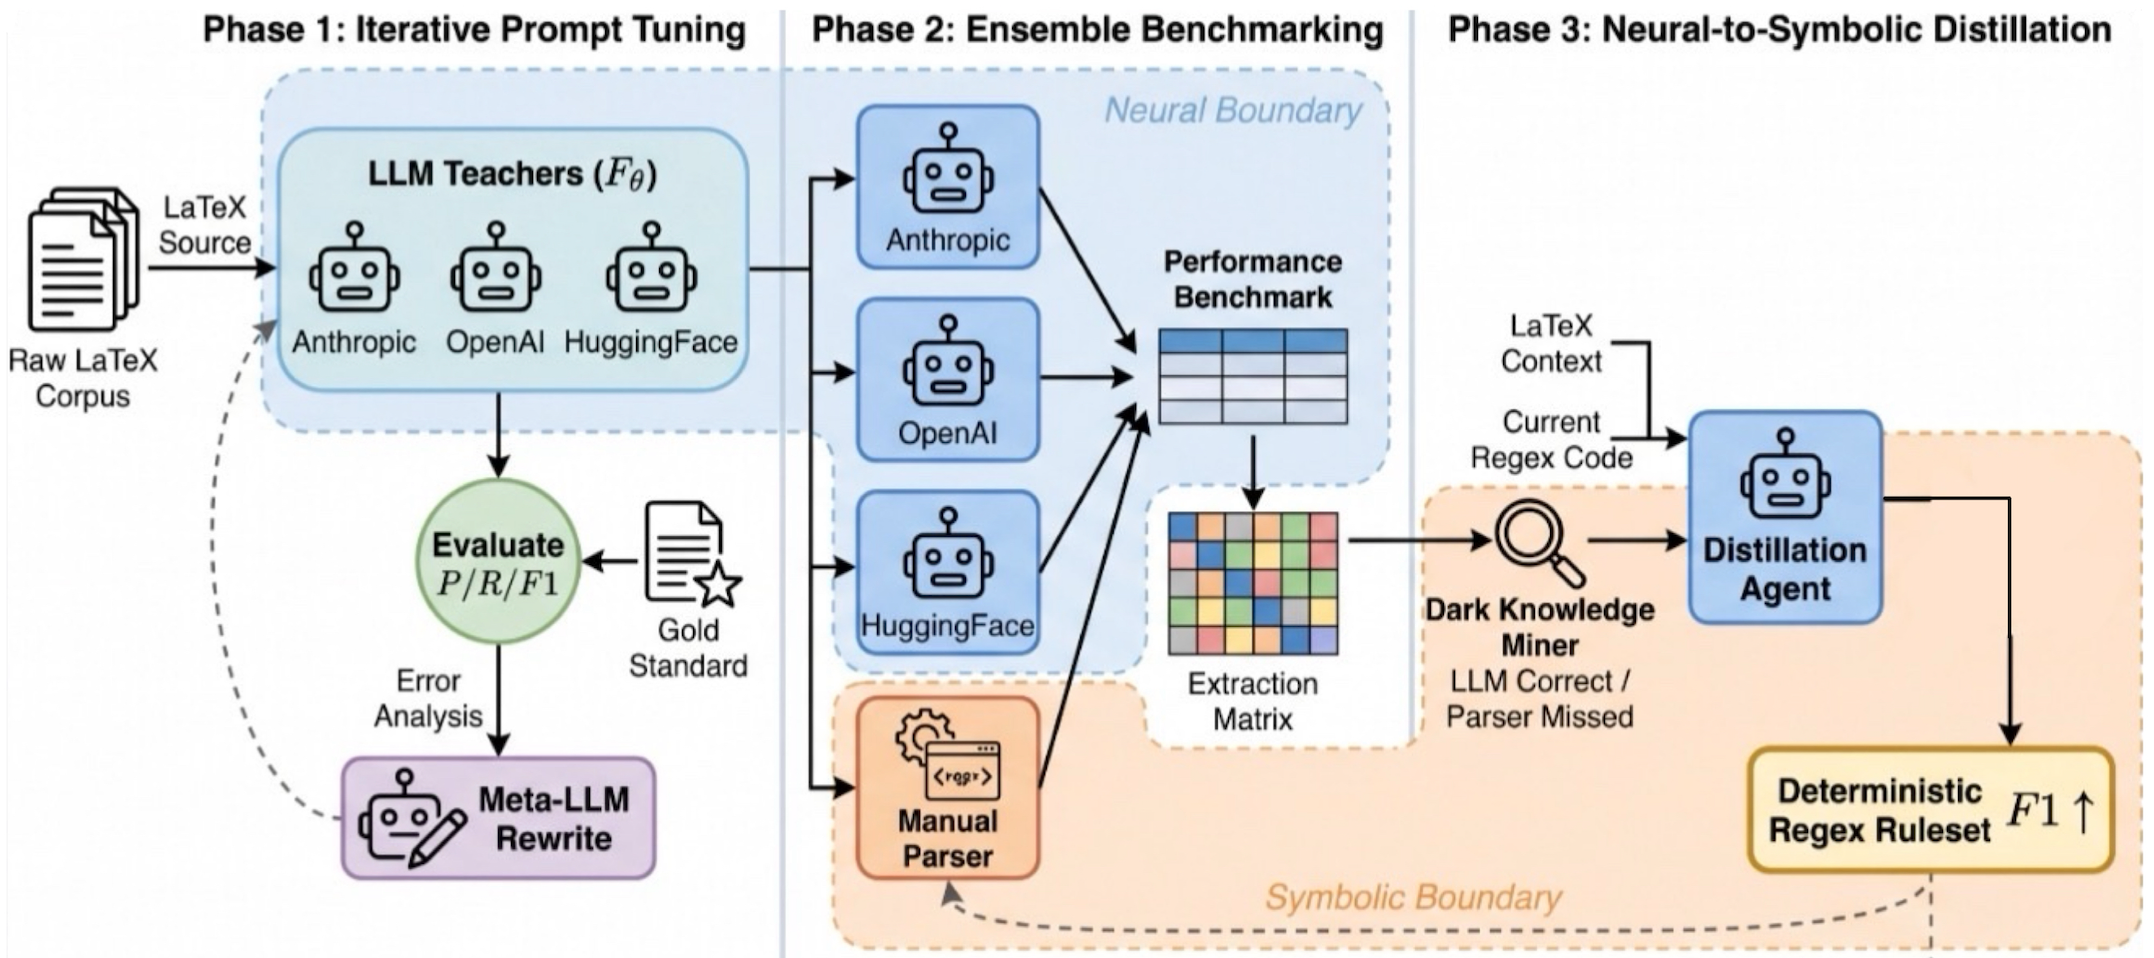
\includegraphics[width=\textwidth]{full pipeline.png}
  \caption{NtRED instantiated for mathematical structure extraction: full pipeline overview
    (teacher optimisation $\to$ ensemble benchmarking $\to$ neural-to-symbolic distillation).}
  \label{fig:pipeline}
\end{figure}

\begin{figure}[h]
  \centering
  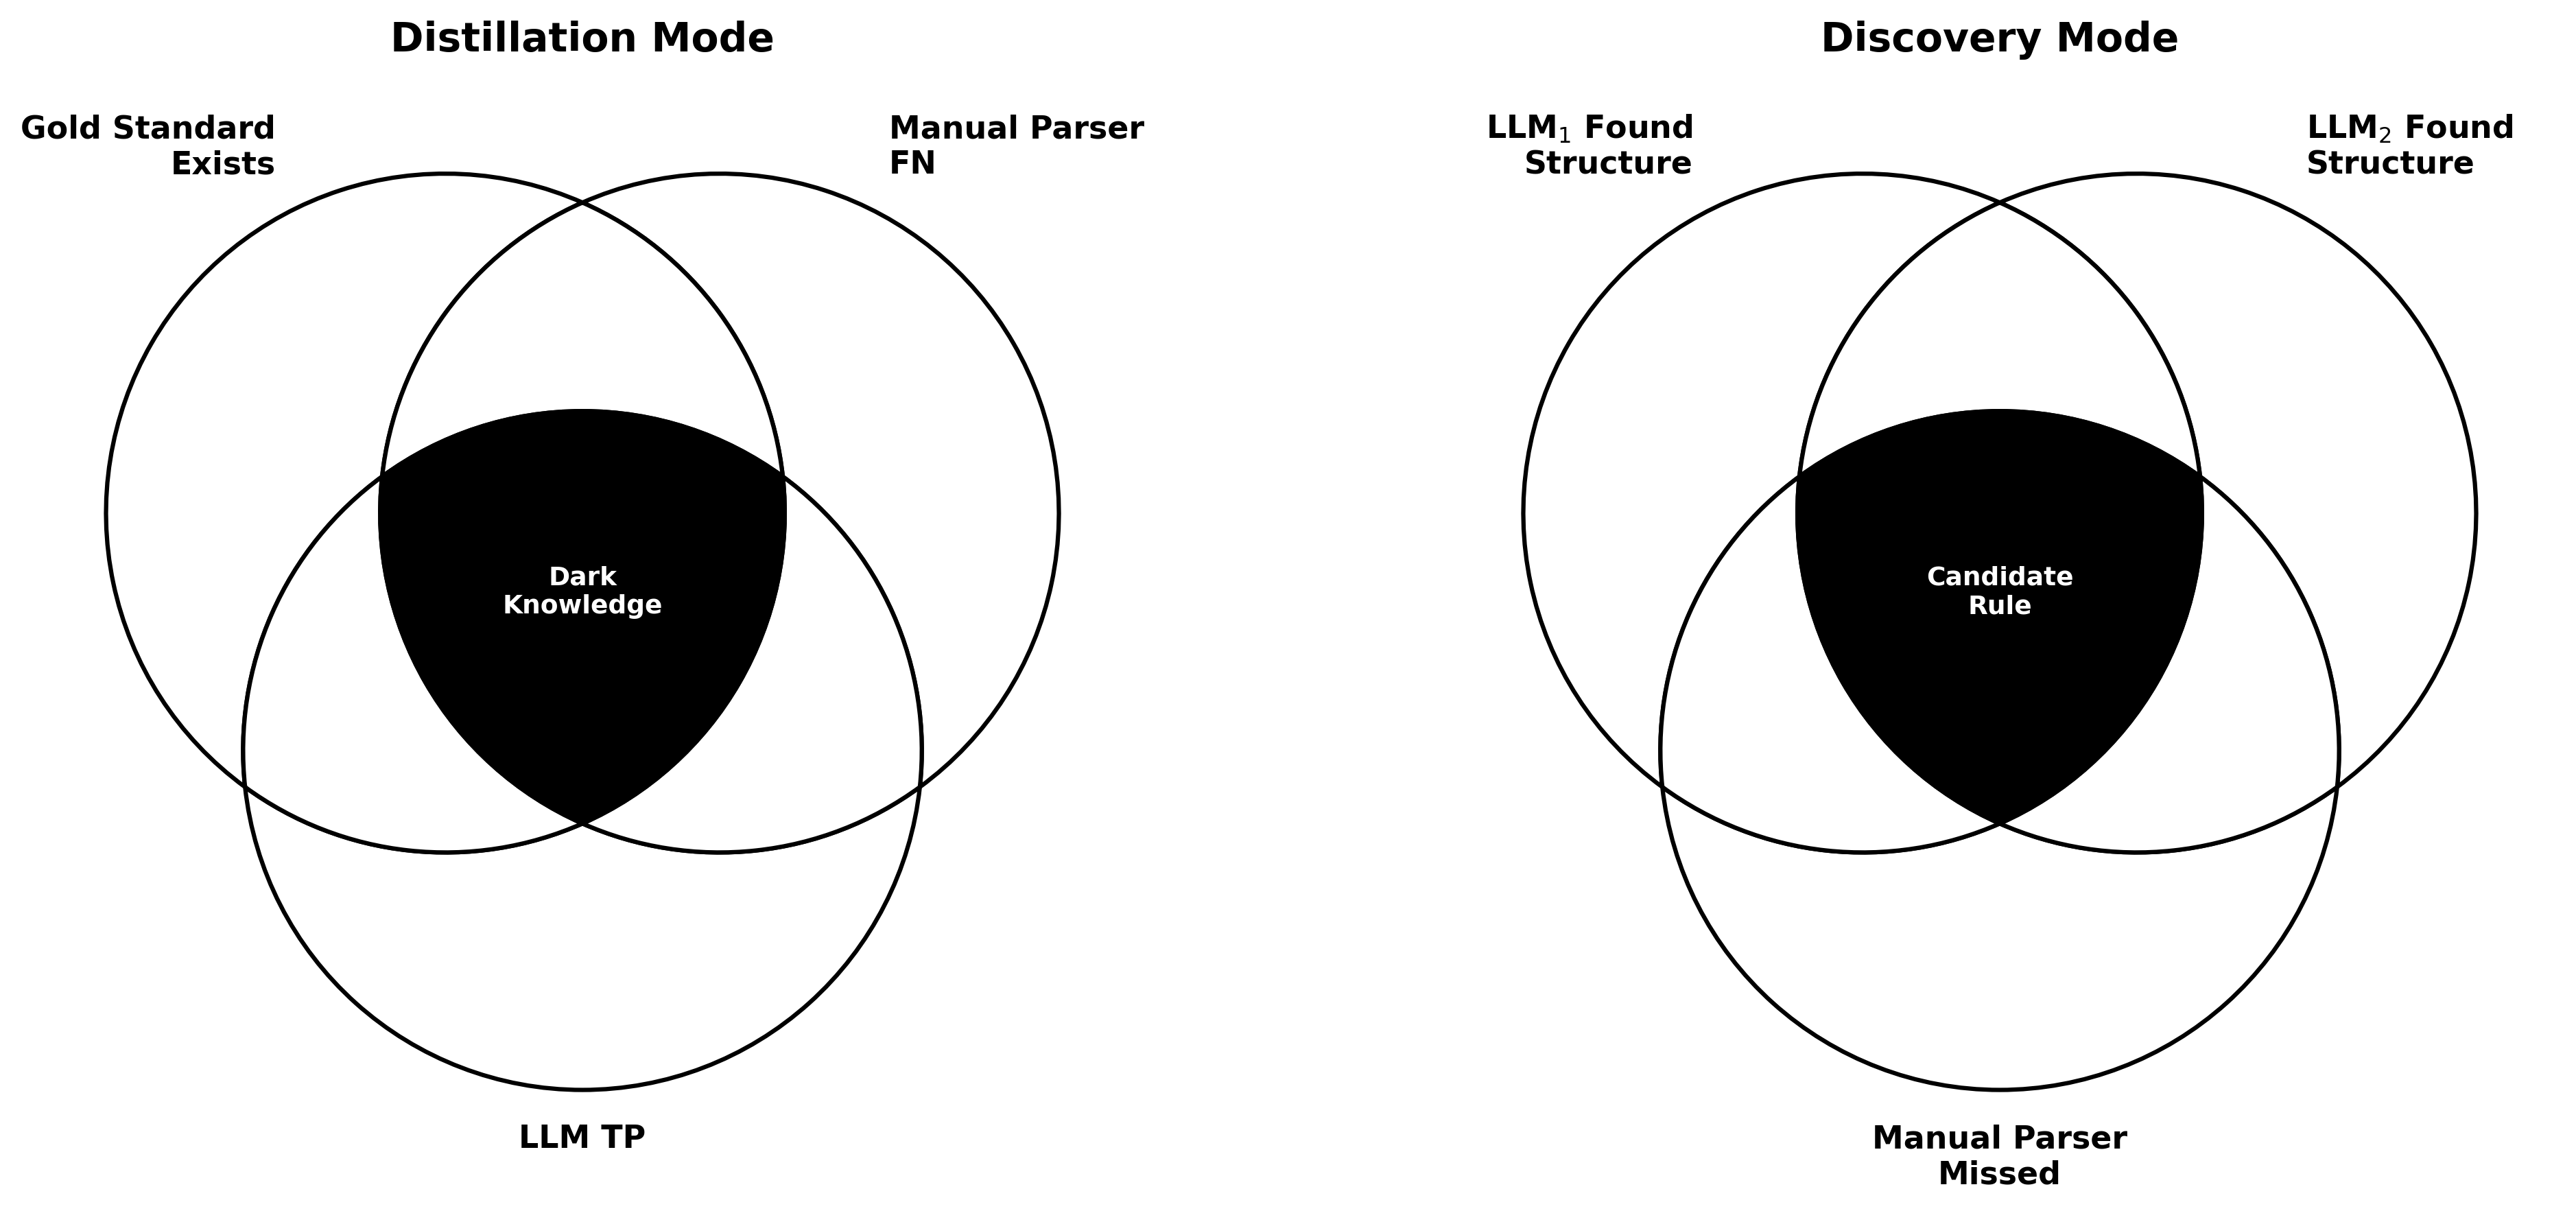
\includegraphics[width=0.55\textwidth]{venn_modes.png}
  \caption{Operating modes of NtRED: distillation mode (gold-labelled corpus, left) uses the
    gold standard as ground truth; discovery mode (unlabelled corpus, right) replaces it with
    multi-teacher consensus ($\tau \geq 2$).}
  \label{fig:venn}
\end{figure}

\begin{thebibliography}{1}
\bibitem{hinton2015}
G.~Hinton, O.~Vinyals, and J.~Dean.
\newblock Distilling the knowledge in a neural network.
\newblock \emph{NIPS Deep Learning and Representation Learning Workshop}, 2015.
\end{thebibliography}

\appendix
\begingroup
\sffamily  % switch to sans-serif for the entire appendix

\noindent\rule{\textwidth}{0.8pt}\\[2pt]
{\large\bfseries\sffamily Appendix}\\[-4pt]
\noindent\rule{\textwidth}{0.4pt}
\vspace{0.5em}

\section{Teacher Optimisation Algorithm}
\label{app:optimizer}

The optimiser takes an initial extraction prompt and iteratively improves it by learning from
its own errors against a gold-standard corpus (Figure~\ref{fig:algo_opt}).

\paragraph{Setup.}
The process begins with an initial prompt template (default or user-provided), a set of
training papers with known gold-standard extractions, and a Jaccard similarity threshold
$\theta$ (default $0.7$) that defines what counts as a successful match
(Equation~\ref{eq:jaccard}). Two LLMs are involved: an extraction LLM that identifies
structures from paper source, and a meta-LLM that rewrites the prompt between iterations.

\paragraph{Iterative loop.}
Each iteration performs five steps:

\begin{enumerate}
  \item \textbf{Extract.} The current prompt is sent to the extraction LLM together with each
    training paper's \LaTeX\ source. The LLM returns a JSON array of extracted structures.

  \item \textbf{Evaluate.} Each extracted item is matched against gold-standard entries via
    Jaccard similarity (Equation~\ref{eq:jaccard}). An extraction is a true positive if its
    best gold match meets or exceeds $\theta$; unmatched gold items are false negatives;
    extractions with no sufficiently close gold match are false positives. Precision, recall,
    and F1 are computed and micro-averaged across all training papers.

  \item \textbf{Track best.} If the current F1 exceeds the best seen so far, the current
    prompt is saved as the best candidate.

  \item \textbf{Analyse errors.} Match results are partitioned into three buckets: false
    negatives (gold items entirely missed), false positives (extractions with similarity below
    $0.3$ to any gold item), and near-misses (extractions that partially matched but fell
    short of $\theta$). A fixed character budget is distributed across buckets, prioritising
    near-misses by descending similarity, false positives by ascending similarity, and false
    negatives thereafter.

  \item \textbf{Rewrite prompt.} The meta-LLM receives the current prompt, evaluation
    metrics, and error examples from all three buckets alongside a small set of gold-standard
    samples for reference. It returns a revised prompt with reasoning.
\end{enumerate}

\paragraph{Output.}
The best prompt (by training F1) is written to disk. The best prompt is then evaluated against
a held-out validation set; validation papers are never used during error analysis or prompt
rewriting, providing an unbiased estimate of generalisation and guarding against
paper-specific overfitting.

\begin{figure}[h]
  \centering
  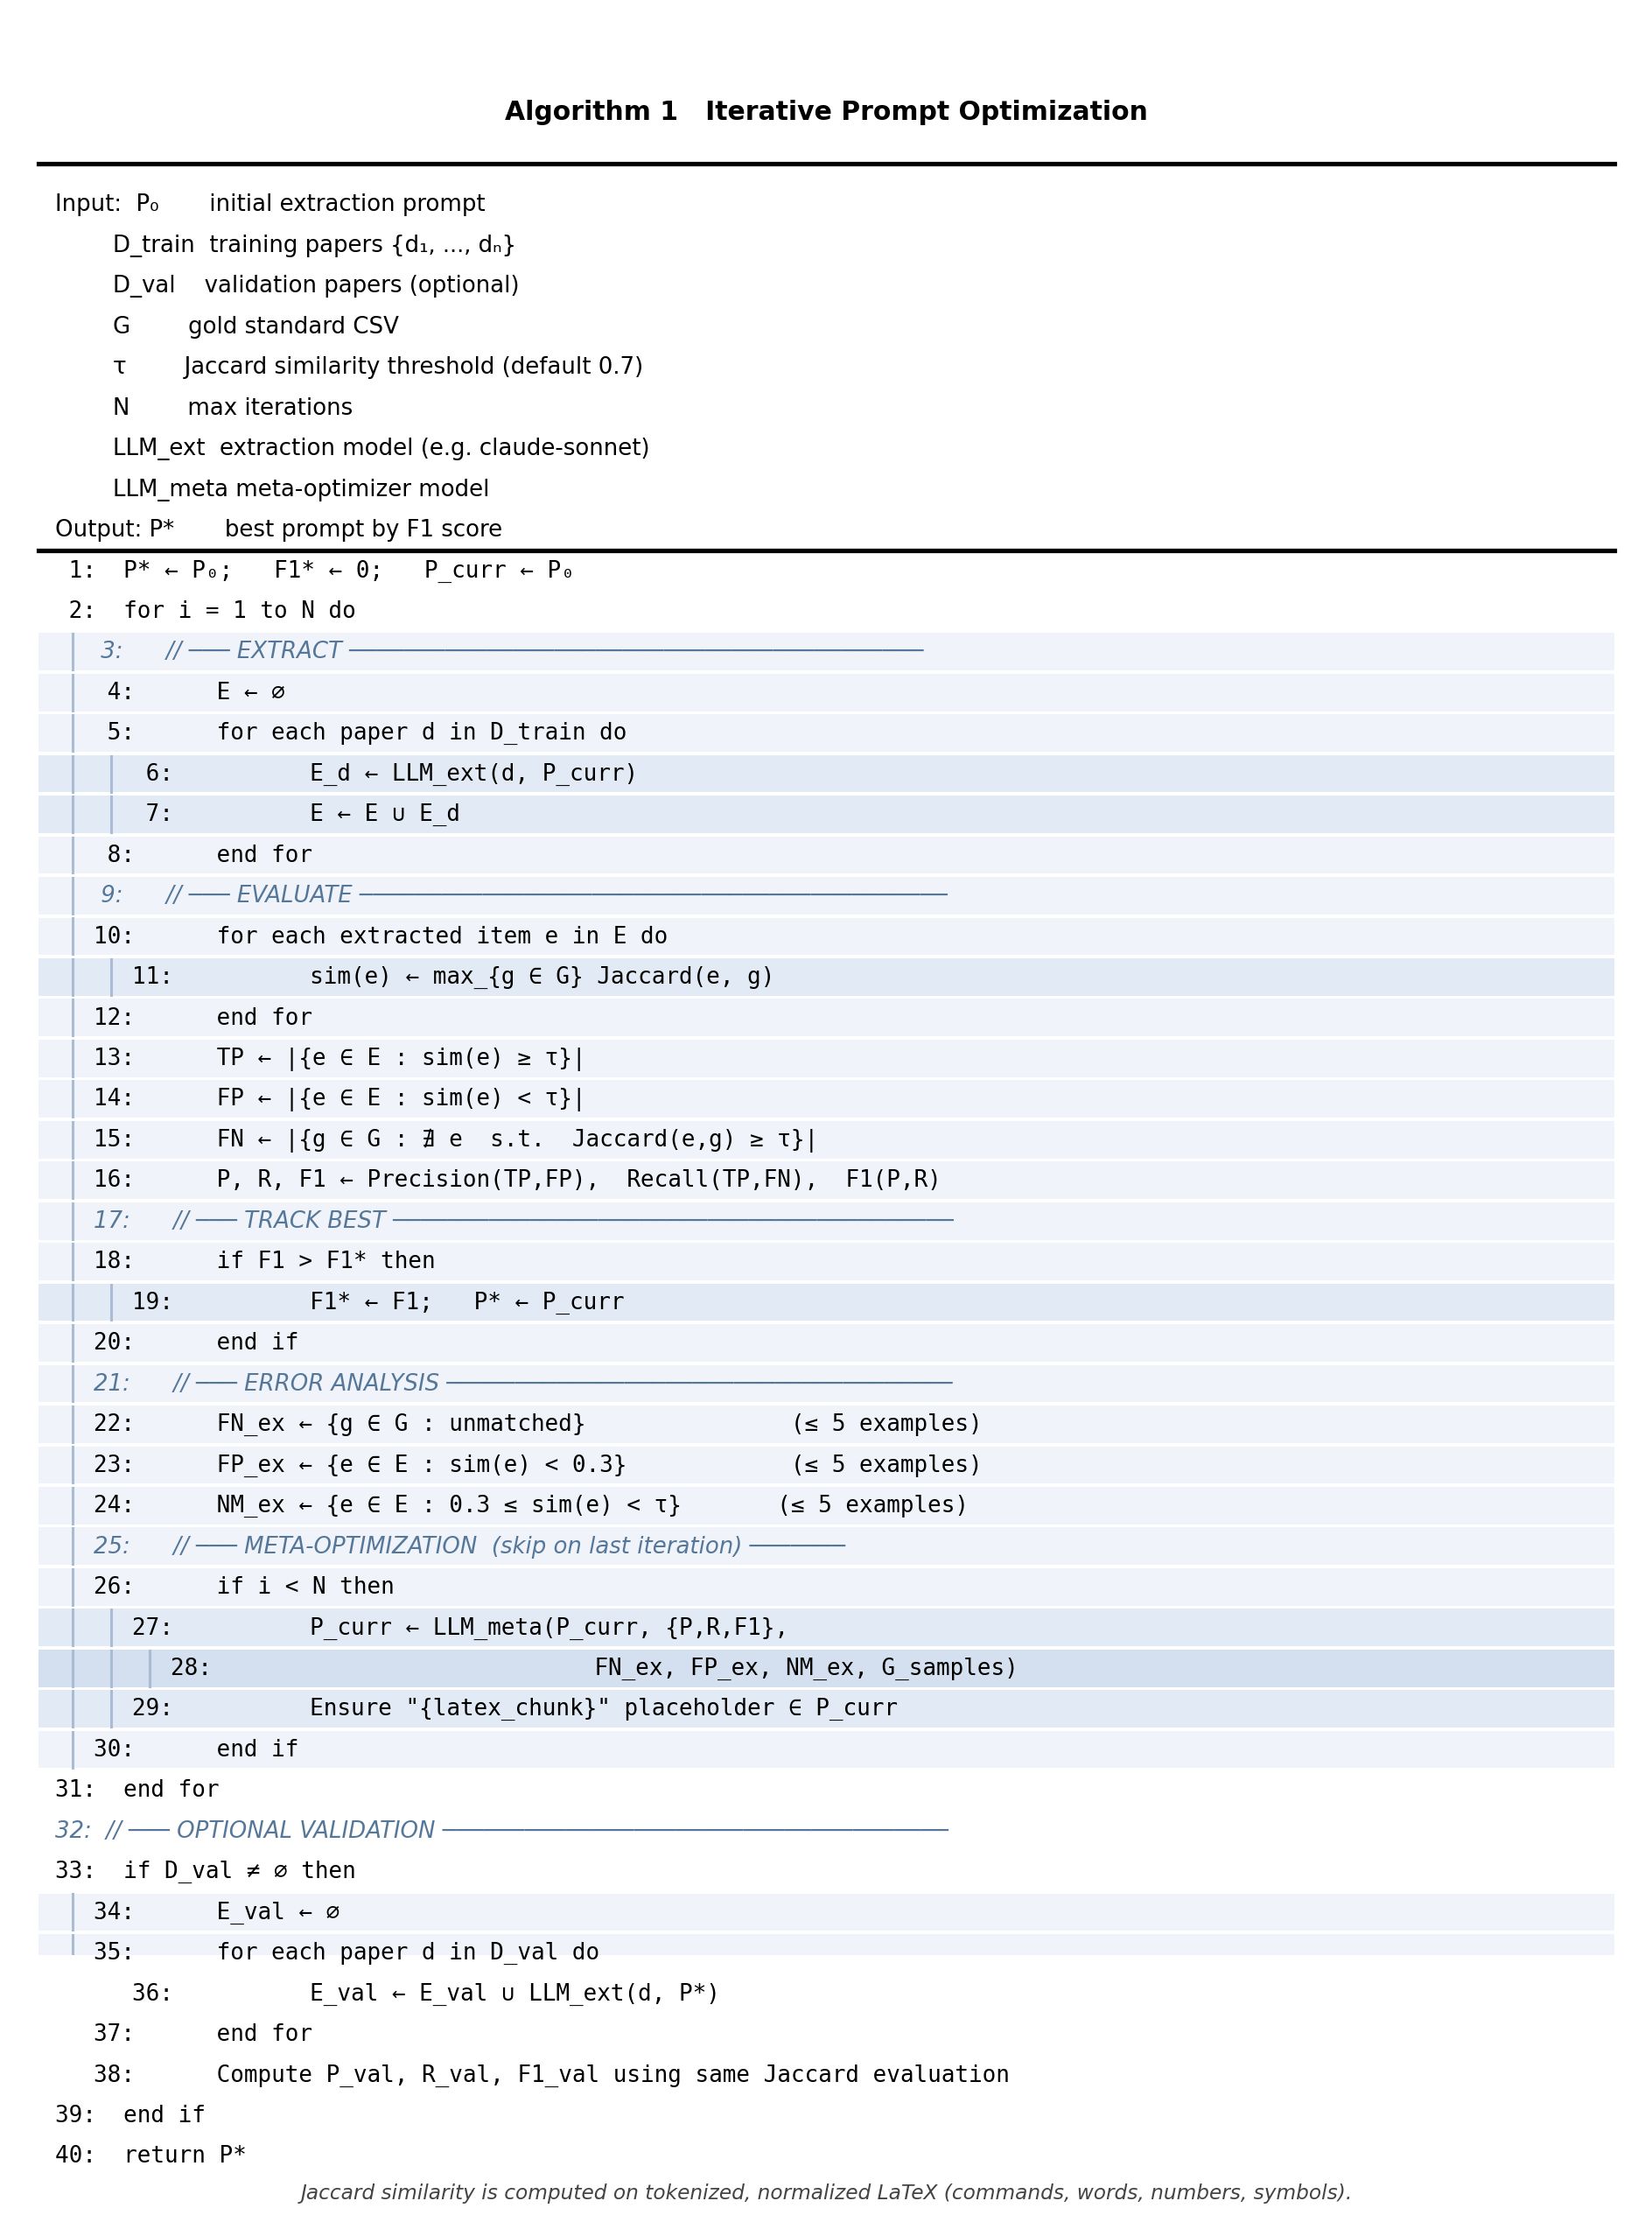
\includegraphics[width=0.5\textwidth]{algorithm_optimization.png}
  \caption{Pseudocode for the teacher optimisation loop (Phase~I), instantiated for
    mathematical structure extraction from \LaTeX\ source.}
  \label{fig:algo_opt}
\end{figure}

\section{Prompt Optimisation Example: Definition Extraction}
\label{app:prompt_example}

Figure~\ref{fig:prompt_opt_example} shows a concrete example of the teacher optimisation
process applied to the definition extraction prompt for the Anthropic provider. The left
column shows the \emph{initial prompt}---a concise instruction to identify mathematical
definitions from \LaTeX\ source. The right column shows the \emph{optimised prompt} after
three iterations of the loop described in Appendix~\ref{app:optimizer}.

\begin{figure}[h]
  \centering
  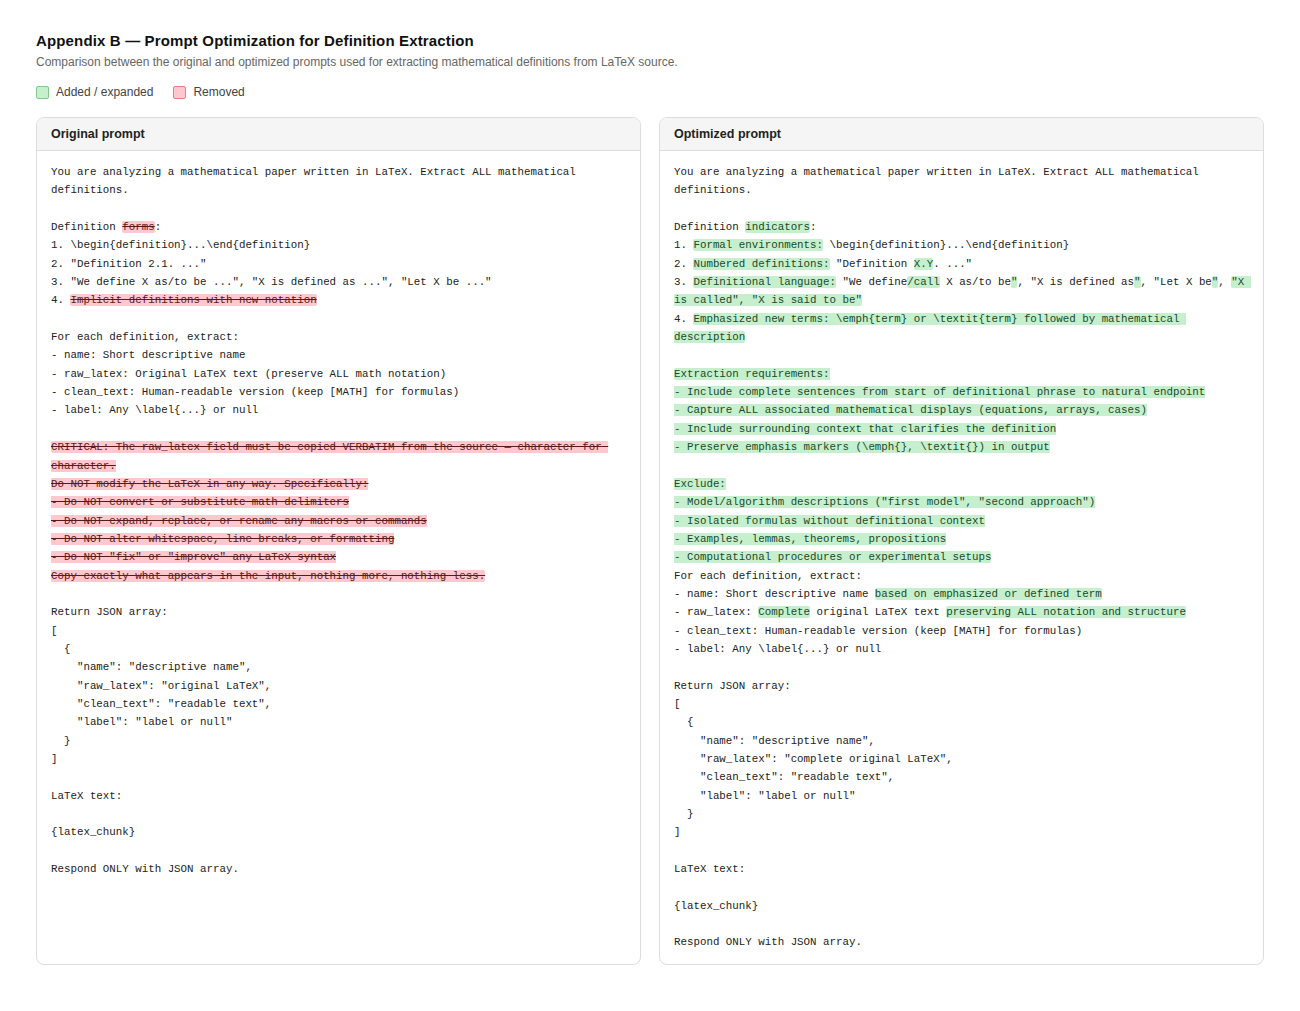
\includegraphics[width=\textwidth]{prompt_opt_example.png}
  \caption{Initial vs.\ optimised extraction prompt for mathematical definitions (Anthropic
    provider, three optimisation iterations). Additions introduced by the meta-LLM are
    highlighted in green; deleted text in red.}
  \label{fig:prompt_opt_example}
\end{figure}

\endgroup  % end sans-serif appendix group

\end{document}
